% EEE3094S Lab 2 report. Rules from the 2026 brief, keep them in view:
%   15 pages max excluding cover, contents and appendices. 10 percent penalty over.
%   A 10 page report is what the brief calls perfect for this scope.
%   No photos of handwritten work, no Excel plots.
%   Every figure captioned, annotated, and referred to in the text.
%   Demo screenshot of the controller tracking the setpoint goes in the appendix.
%   Sections below match the rubric: System Identification 20, Controller Design,
%   Controller Tests, and the modelling that feeds them.
% Build: latexmk -pdf main.tex

\documentclass[11pt,a4paper]{article}

\usepackage[utf8]{inputenc}
\usepackage[english]{babel}

\usepackage[pdftex]{graphicx}
\usepackage{amsmath}
\usepackage{booktabs}
\usepackage[top=0.9in, bottom=0.9in, left=0.95in, right=0.95in]{geometry}

\linespread{1.0}
\setlength{\parskip}{5pt plus2pt minus1pt}

\widowpenalty 10000
\clubpenalty 10000

\newcommand{\eat}[1]{}
\newcommand{\HRule}{\rule{\linewidth}{0.5mm}}

\usepackage[official]{eurosym}
\usepackage{enumitem}
\setlist{nolistsep,noitemsep}
\usepackage[hidelinks]{hyperref}

% pack floats with text instead of letting them take whole pages
\renewcommand{\topfraction}{0.92}
\renewcommand{\bottomfraction}{0.80}
\renewcommand{\textfraction}{0.06}
\renewcommand{\floatpagefraction}{0.85}
\setcounter{topnumber}{3}
\setcounter{bottomnumber}{2}
\setcounter{totalnumber}{5}

% tighter display-equation and float spacing, to stay inside the 15 page limit
\setlength{\abovedisplayskip}{5pt plus 2pt minus 2pt}
\setlength{\belowdisplayskip}{5pt plus 2pt minus 2pt}
\setlength{\abovedisplayshortskip}{3pt plus 1pt minus 1pt}
\setlength{\belowdisplayshortskip}{3pt plus 1pt minus 1pt}
\setlength{\textfloatsep}{8pt plus 2pt minus 2pt}
\setlength{\intextsep}{8pt plus 2pt minus 2pt}
\setlength{\floatsep}{8pt plus 2pt minus 2pt}

% Bibliography needs biber, which is not installed on this machine. Uncomment both
% lines plus % \printbibliography below once you actually cite something.
% \usepackage[backend=biber,style=alphabetic,sorting=ynt]{biblatex}
% \addbibresource{Bibliography.bib}

\begin{document}

\begin{titlepage}
\begin{center}


\includegraphics[width=0.3\textwidth]{UCTLOGO.png}~\\[2cm]

\HRule \\[0.4cm]
{ \LARGE
  \textbf{Lab 2 Report}\\[0.4cm]
  \emph{Proportional Control}\\[0.4cm]
}
\HRule \\[1.5cm]

{ \large
  Tri Tac Le\\[0.2cm]
  EEE3094S Control Systems Engineering\\[0.2cm]
  LXXTRI004
}

\vfill

\textsc{\large Mechatronics, Department of Electrical Engineering}\\[0.4cm]
{\large \today}

\end{center}
\end{titlepage}

% Sits before the page counter is reset, so it must not print a number of its own.
\thispagestyle{empty}
\section*{Declaration}

\begin{enumerate}
    \item I know that plagiarism is a serious form of academic dishonesty.
    \item I have read the document about avoiding plagiarism, am familiar with its contents
          and have avoided all forms of plagiarism mentioned there.
    \item Where I have used the words of others, I have indicated this by the use of
          quotation marks.
    \item I have referenced all quotations and properly acknowledged other ideas borrowed
          from others.
    \item I have not and shall not allow others to plagiarise my work.
    \item I declare that this is my own work.
\end{enumerate}

\vspace{1.5em}

\noindent Name: Tri Tac Le \hfill Student number: LXXTRI004

\vspace{2.5em}

\noindent Signature: Tri Tac Le \hfill Date: \today

\newpage


\tableofcontents
\thispagestyle{empty}
\newpage

\pagenumbering{arabic}

\section{Introduction}\label{sec:intro}
This lab builds a proportional controller for a simulated kitticopter and tests it on the real
system. The kitticopter moves vertically under rotor thrust, aerodynamic drag and gravity, and
its parameters are unique to each student, so the model cannot be taken from the brief and has
to be measured.

The work runs over two lab sessions. The first identifies the system: the hover voltage is
found, a step test is run at the input, and the resulting response gives the plant gain $A$, the
time constant $T$ and the sensor constant $k$. The second designs a proportional controller from
those parameters, builds it on Veroboard from op-amp stages, and demonstrates it tracking a
position setpoint.

The controller has to track position setpoints to within $8$ percent, keep overshoot below $30$
percent, and hold both of those in the face of $10$ percent uncertainty in the aerodynamic
constant and $10$ percent tolerance in the components used to build it. This report derives the
model, reports the measurements and the parameters extracted from them, shows how the gain was
chosen against those four specifications, and evaluates what the built controller actually
achieved.

\section{System Modelling}\label{sec:modelling}
The kitticopter is a single mass moving vertically under three forces: rotor thrust, aerodynamic
drag and gravity. This section builds the model that the rest of the report rests on. It starts
from the forces, reaches a differential equation, and converts that equation into the transfer
functions used to design the controller. The model is left in terms of three constants that
cannot be derived from the brief and have to be measured on the system itself: the plant gain
$A$, the time constant $T$ and the sensor constant $k$. Section~\ref{sec:system_id} measures
them.

\subsection{Forces on the kitticopter}
Figure~\ref{fig:fbd} shows the three forces. Upwards is taken as positive, so the position
$y(t)$, the velocity $\dot{y}(t)$ and the thrust $f_t(t)$ are all positive upwards, while weight
acts downwards and drag acts against whichever way the kitticopter is moving.

\begin{figure}[htbp]
    \centering
    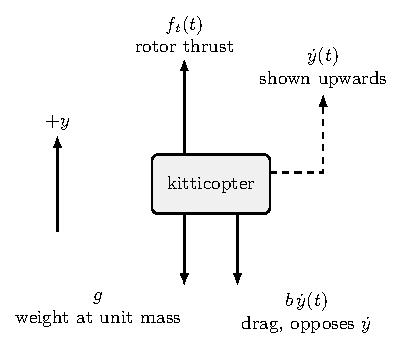
\includegraphics[width=0.34\textwidth]{figures/fbd.pdf}
    \caption{Free-body diagram of the kitticopter. Rotor thrust $f_t$ acts upwards, weight $g$
    acts downwards, and drag $b\dot{y}$ opposes the velocity. Upwards is positive.}
    \label{fig:fbd}
\end{figure}

Three modelling decisions come from the brief and each is used later.

\begin{enumerate}
    \item \textbf{Everything is normalised to the mass.} Newton's second law reads
    $m\ddot{y} = f_t - b_{\text{phys}}\dot{y} - mg$; dividing by $m$ and setting $m = 1$ folds
    the mass into every coefficient, so the thrust term is already an acceleration, $b$ has
    units of $\mathrm{s^{-1}}$ and $a$ has units of $\mathrm{m\,s^{-2}}$ per volt. Without
    stating this the units in the transfer function do not balance.
    \item \textbf{Drag is proportional to velocity and opposes it.} This keeps the model linear
    and first order in velocity, which is what makes it identifiable from a step test.
    \item \textbf{Gravity is a constant disturbance at the input.} It depends on neither position,
    velocity nor thrust, so it adds a fixed term to the acceleration rather than to the dynamics.
    That is why a fixed bias cancels it, and why the controller output is offset by the hover
    voltage rather than starting from zero.
\end{enumerate}

\subsection{Equation of motion}
Summing the forces of Figure~\ref{fig:fbd} at unit mass gives the acceleration of the
kitticopter,
\begin{equation}\label{eqn:eom}
    \ddot{y}(t) = a\,f_t(t) - b\,\dot{y}(t) - g ,
\end{equation}
with $g = 9.81\ \mathrm{m\,s^{-2}}$. The minus sign on the drag term is the statement that drag
opposes motion, and the minus sign on $g$ is the sign convention of Figure~\ref{fig:fbd}. Both
$a$ and $b$ are unknown at this stage.

\subsection{The controlled system and its interfaces}
The kitticopter is simulated while the controller is a physical circuit, so the loop crosses
between the two twice. The command is a voltage setting the angle of attack of the rotor blades,
entering through an ADC that accepts $0$ to $5\ \mathrm{V}$ with the midpoint calibrated to the
thrust that cancels gravity. Position leaves through a DAC and the sensor constant $k$, and since
the summing junction compares voltages, the same $k$ converts the setpoint from metres to volts.

\begin{figure}[htbp]
    \centering
    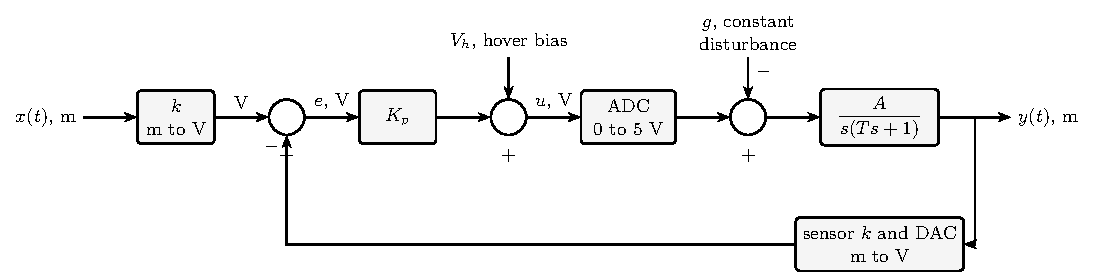
\includegraphics[width=0.85\textwidth]{figures/blockdiagram.pdf}
    \caption{Block diagram of the closed loop. The setpoint $x(t)$ in metres is converted to
    volts by $k$, compared with the fed-back sensor voltage, and the error is amplified by
    $K_p$. The hover bias $V_h$ is added at a separate summing junction so that the command
    $u(t)$ sits inside the $0$ to $5\ \mathrm{V}$ window the plant accepts. Gravity enters as a
    constant disturbance at the plant input, the same node the command arrives at.}
    \label{fig:blockdiagram}
\end{figure}

Two features of Figure~\ref{fig:blockdiagram} are used throughout. Gravity is summed at the plant
\emph{input}, not the output, and the level shift is its own summing junction rather than being
folded into $K_p$. Keeping it separate is what lets the gain be chosen on dynamic grounds alone
while the bias is trimmed independently.

\subsection{Transfer functions}
\subsubsection{Open loop}
Let $v = \dot{y}$ and treat gravity as the disturbance it is. Equation~\eqref{eqn:eom} then
reduces to $\dot{v} = a f_t - b v$, and with zero initial conditions,
\begin{equation}\label{eqn:openloop_vel}
    \frac{V(s)}{F_t(s)} = \frac{a}{s + b} = \frac{A}{Ts + 1},
    \qquad A = \frac{a}{b}, \qquad T = \frac{1}{b} .
\end{equation}

Working at velocity level is deliberate. At position level the pole at the origin means a step
drives the output away without settling, so there is no steady state from which to read a gain.
Differentiating the position gives Equation~\eqref{eqn:openloop_vel}, which has a finite final
value, so one step test fixes both unknowns: the gain from the settled velocity, the time constant
from how fast it is reached.

Position follows by integrating the velocity, which returns the pole at the origin:
\begin{equation}\label{eqn:openloop_pos}
    G(s) = \frac{Y(s)}{F_t(s)} = \frac{A}{s(Ts + 1)} .
\end{equation}

\subsubsection{Closed loop}
With gain $K_p$ and the sensor constant $k$ on both the feedback path and the reference
conversion, the loop gain is
\begin{equation}\label{eqn:loopgain}
    L(s) = \frac{K_p k A}{s(Ts + 1)} ,
\end{equation}
and the closed loop from setpoint to position, both in metres, is
\begin{equation}\label{eqn:closedloop}
    G_{cl}(s) = \frac{Y(s)}{X(s)} = \frac{K_p k A}{Ts^2 + s + K_p k A} .
\end{equation}

Dividing through by $T$ puts Equation~\eqref{eqn:closedloop} in the standard second-order form
$\omega_n^2 / (s^2 + 2\zeta\omega_n s + \omega_n^2)$, from which
\begin{equation}\label{eqn:wn_zeta}
    \omega_n = \sqrt{\frac{K_p k A}{T}},
    \qquad
    \zeta = \frac{1}{2\sqrt{T K_p k A}} .
\end{equation}

Equation~\eqref{eqn:wn_zeta} is the whole design problem in one line. Once the plant is
measured, $K_p$ is the only free parameter, and raising it raises $\omega_n$ while lowering
$\zeta$. Speed and overshoot therefore trade directly against one another, and
Section~\ref{sec:design} does nothing more than find the range of $K_p$ where both stay inside
the specification.

\subsection{Error, disturbance and type number}
The open loop of Equation~\eqref{eqn:openloop_pos} carries one free integrator, so the system is
type 1, and the final value theorem fixes two things before any gain is chosen. A step setpoint is
tracked with zero steady-state error, so the tracking half of the $8$ percent specification is met
by the structure rather than by tuning. A constant input disturbance, which is what gravity is,
leaves a finite offset
\begin{equation}\label{eqn:fvt_dist}
    y_{ss} = \frac{\Delta V}{K_p k} ,
\end{equation}
per volt of uncancelled input. No $K_p$ removes it, which is why the level shift exists and why
the whole $8$ percent budget is spent on the disturbance. Both closed-loop transfer functions are
derived in Appendix~\ref{sec:appendix}.

The structure is fixed; three constants are not. The gain $A$, the time constant $T = 1/b$ set by
drag, and the sensor constant $k$ are unique to this kitticopter.
Section~\ref{sec:system_id} measures them and Section~\ref{sec:design} uses them in
Equation~\eqref{eqn:wn_zeta} to choose $K_p$.

\section{System Identification}\label{sec:system_id}
Section~\ref{sec:modelling} left three constants unmeasured: the plant gain $A$, the time constant
$T$ and the sensor constant $k$. This section reports the tests that fixed them.

\subsection{Method}
The plant is first order at velocity level and second order at position level, so the tests are
built around Equation~\eqref{eqn:openloop_vel} rather than Equation~\eqref{eqn:openloop_pos}.

\paragraph{Hover voltage.} The input was raised until the kitticopter held height with its
vertical speed below $0.02\ \mathrm{m\,s^{-1}}$, where thrust exactly cancels gravity. This is the
zero point of the controller and the baseline of every step test; stepping from $0\ \mathrm{V}$
would start the kitticopter in free fall and the trace would not be a step response of the linear
model. Measured twice, at $2.495$ and $2.515\ \mathrm{V}$.

\paragraph{Input circuit.} Steps were commanded from a breadboard divider off the
$15\ \mathrm{V}$ rail: $56\ \mathrm{k\Omega}$ to a trimmer, $12\ \mathrm{k\Omega}$ to ground,
wiper to ADC input 1. Its range is bounded to keep the command inside the $0$ to $5\ \mathrm{V}$
window the plant accepts, since above $5\ \mathrm{V}$ the excess is ignored and the commanded step
would be larger than the one the plant actually saw.

\paragraph{Velocity.} The rig logs time, input voltage, output voltage and position, but no
velocity, so velocity comes from differentiating the logged position with a centred difference,
\begin{equation}\label{eqn:central_difference}
    v_n = \frac{h_{n+1} - h_{n-1}}{t_{n+1} - t_{n-1}} .
\end{equation}
at a $100\ \mathrm{ms}$ sample interval.

\paragraph{Extraction.} From each settled response the gain is the ratio of final velocity to step
size, and the time constant the time to reach $63.2$ percent of that final value:
\begin{equation}\label{eqn:AT_extraction}
    A = \frac{v_\infty}{V_2 - V_h},
    \qquad
    v(T) = 0.632\,v_\infty .
\end{equation}
A second estimate of $T$ comes from fitting a straight line to $\ln(v_\infty - v)$ against time,
whose slope is $-1/T$. The two estimates are reported together as a check on each other.

\paragraph{Sign of the difference.} Equation~\eqref{eqn:central_difference} is signed, not a
magnitude. A climb gives a positive velocity and a fall a negative one, and the decay tests depend
on that: absolute values would fold the decay back on itself and make the fitted time constant
meaningless.

\paragraph{Choice of interval.} The differencing interval is a judgement rather than a constant,
and it was chosen differently in different parts of each run. The logged position is quantised, so
over one $100\ \mathrm{ms}$ sample that quantisation is a significant fraction of the few metres
travelled and the velocity is noisy; widening the interval averages it away, because the same
quantisation is negligible against a change of hundreds of metres. But a wide interval also
averages across curvature, and during the transient the curvature is the signal being measured.

The resolution is to match the interval to the region. On the settled plateau the curve is
straight, so tens of seconds are used, which is what Equation~\eqref{eqn:dhdt_worked} does.
Through the transient a centred difference over neighbouring samples is used instead and the extra
noise accepted. One interval everywhere would either corrupt the plateau with noise or flatten
the transient, and both errors land directly on $A$ and $T$.

\paragraph{Gain from a regression, not a single run.} Each run on its own gives a gain by
Equation~\eqref{eqn:AT_extraction}, but that ratio assumes the hover voltage is exactly right: an
error in $V_h$ shifts every step size by the same amount and biases the gain. Fitting the settled
velocities of all the runs against input voltage instead removes the assumption and returns the
hover voltage as a result, as Equation~\eqref{eqn:gain_regression} does.

\paragraph{Time constant from the position curve, not the velocity curve.} Reading the $63.2$
percent level requires a velocity signal, which requires differentiating the log and therefore
amplifying its quantisation. Fitting the analytic position response of
Equation~\eqref{eqn:height_fit} instead uses the raw logged column with no differentiation at all,
and uses every sample rather than the single crossing point. It is the better conditioned of the
two routes, so it is the one reported, with the $63.2$ percent reading kept as the check.

\paragraph{Decay tests as validation, not as measurement.} In a step test $A$ and $T$ are pulled
from the same curve, so an error in one can hide inside the other and the fit still looks good.
Stepping the input back down to hover breaks that coupling: the velocity decays toward zero, there
is no final value for the gain to influence, and what remains depends on $T$ alone. That is why
the decay result is reported as a check on the model rather than averaged into it.

\subsection{Results}
Eight runs are used: seven step tests at four step sizes, with the two smallest and the largest repeated, plus the full-range test of Section~\ref{sec:system_id}.
Table~\ref{tab:stepruns} lists them. Figure~\ref{fig:step_response} shows the velocity responses
aligned at the step, and the linearity check described below.


\begin{figure}[htbp]
    \centering
    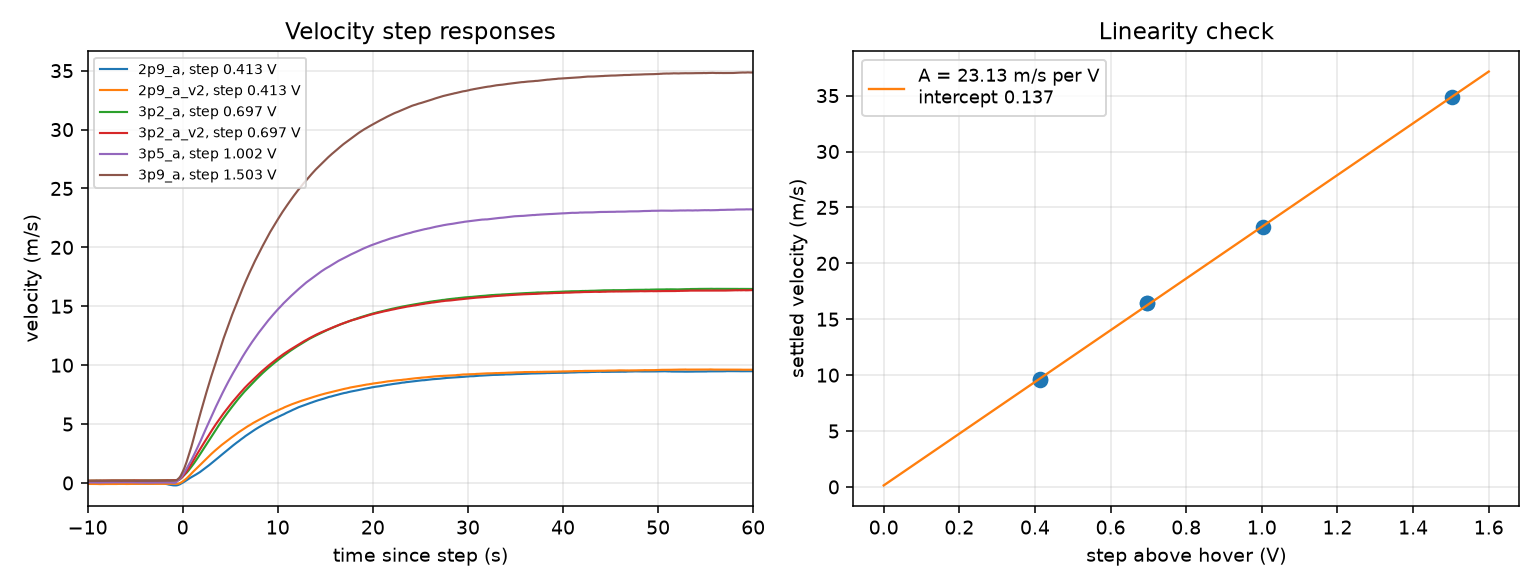
\includegraphics[width=0.62\textwidth]{figures/step_response.png}
    \caption{Left: velocity against time for the seven step runs, aligned at the instant of the step.
    Each settles to a constant, as a first-order response should, with no overshoot. Right:
    settled velocity against raw input voltage. The straight line has slope $23.196$ and crosses
    zero velocity at $2.5016\ \mathrm{V}$, recovering the hover voltage without it having been
    assumed.}
    \label{fig:step_response}
\end{figure}

\paragraph{Gain and hover voltage from one fit.} The individual ratios in
Table~\ref{tab:stepruns} each divide by $V_{in} - V_h$, so each one inherits whatever error is in
the hover voltage. Regressing the settled velocity against the \emph{raw} input voltage removes
that dependence, because

\begin{equation}
    v_\infty = A\left(V_{in} - V_h\right) = A\,V_{in} - A V_h ,
\end{equation}
so the slope is the gain and the horizontal intercept is the hover voltage. Neither is assumed;
both are fitted. Over the eight runs,
\begin{align}\label{eqn:gain_regression}\begin{split}
    A = \frac{n\sum V_{in}v_\infty - \sum V_{in} \sum v_\infty}
             {n \sum V_{in}^2 - \left(\sum V_{in}\right)^2}
      = \frac{8(797.959) - (28.6512)(200.379)}{8(106.0741) - (28.6512)^2} \\
      = \frac{642.572}{27.7015}
      = 23.196\ \mathrm{m\,s^{-1}V^{-1}} ,
\end{split}\end{align}
\begin{equation}
    V_h = -\frac{c}{A} = \frac{58.0278}{23.196} = 2.5016\ \mathrm{V} .
\end{equation}
The residuals are $+0.020$, $-0.023$, $-0.029$, $+0.015$, $-0.008$, $+0.040$, $+0.005$ and
$-0.019\ \mathrm{m\,s^{-1}}$, an rms of $0.022$ against velocities reaching $57.9$. Two things
follow. The plant is linear over the whole $0$ to $5\ \mathrm{V}$ range, since one straight line
fits a sixfold spread of step sizes to within the logging resolution. And the fitted hover voltage
lands on $2.50\ \mathrm{V}$, the midpoint of the input range, which the brief states is where
thrust cancels gravity by design. That value was never put into the fit, so its appearance in the
answer is an independent check on the whole measurement rather than a restatement of an
assumption.

\paragraph{Sensor constant.} The rig logs position in both volts and metres, so $k$ follows from
the ratio of the two columns. Only samples below $9.9\ \mathrm{V}$ were used, because the sensor
output saturates at $10\ \mathrm{V}$ near a height of $10.5\ \mathrm{m}$ while the metre column
continues to read truthfully. Every run gives the same value,
\begin{equation}
    k = 0.9500\ \mathrm{V\,m^{-1}} .
\end{equation}

\subsection{Full-range test}
A final test used the largest step the rig allows, from hover straight to the $5\ \mathrm{V}$
ceiling. Pushing the potentiometer hard against its end stop made the input move from $2.967$ to
$5.000\ \mathrm{V}$ within a single $100\ \mathrm{ms}$ sample, so unlike the earlier runs there is
no ramp to distort the early part of the response. It was held for $185\ \mathrm{s}$, by which
point the velocity was flat to three decimals at $57.935\ \mathrm{m\,s^{-1}}$ and the simulator
reported zero lift, the signature of terminal velocity where thrust balances gravity and drag
together.

\paragraph{Reading the velocity.} Applying the interval rule above to the settled region, two
points $29.9\ \mathrm{s}$ apart late in the run give
\begin{equation}\label{eqn:dhdt_worked}
    v = \frac{3341.697 - 2298.690}{2443.7 - 2413.8} = \frac{1043.007}{29.9}
      = 34.88\ \mathrm{m\,s^{-1}} ,
\end{equation}
stable to three figures, against the same quantity computed over one sample, which scatters by
several $\mathrm{m\,s^{-1}}$.

\paragraph{Gain.} With the fitted hover voltage of $2.5016\ \mathrm{V}$,
\begin{equation}
    A = \frac{57.935}{5.0000 - 2.5016} = 23.197 ,
\end{equation}
which agrees with the regression of Equation~\eqref{eqn:gain_regression} to $0.001$. Taking
hover at its design value of exactly $2.5\ \mathrm{V}$ instead gives $23.174$, a difference of
$0.1$ percent, so the choice no longer matters once the hover voltage is fitted rather than
trimmed by eye.

\paragraph{Time constant.} Two routes were used. Reading the $63.2$ percent level off the velocity
curve gives $0.632 \times 57.935 = 36.615\ \mathrm{m\,s^{-1}}$, crossed at $t = 9.542\ \mathrm{s}$
after the step. Alternatively the analytic step response of the position,
\begin{equation}\label{eqn:height_fit}
    h(t) = v_\infty \left( t - T \left( 1 - e^{-t/T} \right) \right) ,
\end{equation}
was fitted by least squares to all $1800$ logged samples, which avoids differentiating the signal
at all and therefore avoids amplifying its noise. That gives $T = 9.537\ \mathrm{s}$ and
$v_\infty = 57.931\ \mathrm{m\,s^{-1}}$, with an rms residual of $0.403\ \mathrm{m}$ against
$9869\ \mathrm{m}$ of travel. The two routes agree to $0.1$ percent.

The fit also shows how sharply $T$ is determined. Holding the fit at $T = 9.50$ raises the
residual to $0.92\ \mathrm{m}$ and at $T = 9.70$ to $3.75\ \mathrm{m}$, so a $2$ percent error in
$T$ is already an order of magnitude worse than the optimum. This matters in
Section~\ref{sec:design}, where the gain window is narrow enough that the plant parameters have to
be trusted to better than the $10$ percent the specification allows for.

\subsection{Model validation}
Two independent checks were made on the identified model.

\paragraph{Decay test.} In a step test the gain and the time constant come from the same curve, so
an error in one can be absorbed by the other. Returning the input to hover breaks that coupling,
because the velocity then decays with no final value for the gain to influence. Both logs recorded
for this turned out to hold the whole bench session rather than one event, with $14$ and $28$
separate input changes, so one was discarded and a single clean $164\ \mathrm{s}$ segment was
fitted from the other, with the final velocity free rather than assumed to be zero. Details are in
Appendix~\ref{sec:appendix}. It gives $T = 9.163\ \mathrm{s}$, rms residual
$0.113\ \mathrm{m\,s^{-1}}$ over $1640$ samples, which is $3.9$ percent below the step-test value
and is carried into the uncertainty below.

The same fit returns a residual velocity of $0.157\ \mathrm{m\,s^{-1}}$, while the input over that
segment averaged $2.5080\ \mathrm{V}$ and the identified constants predict
$23.196 \times (2.5080 - 2.5016) = 0.149\ \mathrm{m\,s^{-1}}$. The two agree to
$0.008\ \mathrm{m\,s^{-1}}$. This is the strongest check in the identification: a small number
predicted from two constants measured elsewhere, in a part of the data that played no part in
measuring them.

\paragraph{Independent reimplementation.} The entire analysis was carried out twice, once in
Python and once in MATLAB, written separately against the same raw logs. The two agree on $A$,
$T$ and $k$ to three decimal places.

\subsection{Identified model}
\begin{equation}\label{eqn:identified}
    A = 23.196\ \mathrm{m\,s^{-1}V^{-1}}, \qquad
    T = 9.537\ \mathrm{s}, \qquad
    k = 0.9500\ \mathrm{V\,m^{-1}} ,
\end{equation}
so the velocity plant of Equation~\eqref{eqn:openloop_vel} and the position plant of
Equation~\eqref{eqn:openloop_pos} become
\begin{equation}
    \frac{V(s)}{F_t(s)} = \frac{23.196}{9.537s + 1},
    \qquad
    G(s) = \frac{23.196}{s\left(9.537s + 1\right)} .
\end{equation}
The corresponding drag constant is $b = 1/T = 0.10485\ \mathrm{s^{-1}}$, and the thrust constant $a = A/T = 2.4322\ \mathrm{m\,V^{-1}s^{-2}}$.

The figures are carried to three decimals because the design window in
Section~\ref{sec:design} is narrow, but the honest uncertainty is wider than that. The gain is now
the better determined of the two: the regression residual is $0.022\ \mathrm{m\,s^{-1}}$ and the
four routes to $A$ span $23.19$ to $23.22$, so $A = 23.20 \pm 0.03$. The time constant is less settled. The height-curve fit gives $9.537\ \mathrm{s}$ and rejects
anything far from it, trebling its residual at $9.60$, while the independent decay fit gives
$9.163$. The two methods therefore disagree by $3.9$ percent, which is larger than either one's own
scatter, so the defensible statement is $T = 9.5 \pm 0.4$ rather than the tighter figure the
step-test fit alone would suggest. The sensor constant is known to four figures. These uncertainties are carried into the
corner analysis of Section~\ref{sec:design}, where the specification requires robustness to
$10$ percent in the drag constant anyway, which is far wider than either.
The model was also submitted to the parameter-check tool of Appendix~A2 of the brief, which
scores it against the values the simulator was generated from. That exercise and its outcome are
reported in Appendix~\ref{sec:appendix}, since it tests the measurement rather than forming part
of it.

\section{Controller Design}\label{sec:design}
The controller is a proportional gain $K_p$ acting on the error between the setpoint and the
measured position, both in volts, with the hover bias added afterwards. This section turns each
specification into a bound on $K_p$, takes the intersection, and then builds the result from
op-amps.

\subsection{Specifications as bounds on the gain}
\paragraph{Overshoot below 30 percent.} For a second-order system,
$OS = \exp\!\left(-\pi\zeta/\sqrt{1-\zeta^2}\right)$, so an overshoot of $0.30$ requires
\begin{equation}
    \zeta \geq \frac{-\ln 0.30}{\sqrt{\pi^2 + \ln^2 0.30}} = 0.358 .
\end{equation}
Substituting $\zeta$ from Equation~\eqref{eqn:wn_zeta} and inverting gives the ceiling
\begin{equation}\label{eqn:kp_os}
    K_p \leq \frac{1}{4\zeta_{\min}^2\,T k A} = \frac{1.951}{T k A} .
\end{equation}

\paragraph{Robustness to 10 percent in the aerodynamic constant.} A drag error does not move $T$
alone. Both $A = a/b$ and $T = 1/b$ are inversely proportional to $b$, so a single error in $b$
scales them together: the product $kAT$ in Equation~\eqref{eqn:kp_os} varies as the \emph{square}
of the error and $\zeta$ as its reciprocal, not its square root. A drag constant $10$ percent low
therefore raises $kAT$ by $21$ percent rather than $10$, and the ceiling is re-evaluated there.
Treating $T$ as the only affected parameter understates the worst corner, by $0.9$ percentage
points of overshoot in this design.

\paragraph{Robustness to 10 percent component tolerance.} A gain stage built from $10$ percent
parts may land $10$ percent above its design value, so the nominal is chosen such that the high
end of the tolerance band still satisfies the previous bound, giving $1.596/(TkA)$.

\paragraph{Tracking within 8 percent.} Equation~\eqref{eqn:fvt_error} showed the steady-state
error to a step setpoint is zero, so the whole $8$ percent budget belongs to the residual
disturbance of Equation~\eqref{eqn:fvt_dist} left after the hover bias is trimmed. For a
setpoint step $X_0$ and a residual input disturbance $d_{res}$,
\begin{equation}
    \frac{d_{res}}{K_p k} \leq 0.08\,X_0
    \qquad \Rightarrow \qquad
    K_p \geq \frac{d_{res}}{0.08\,k\,X_0} ,
\end{equation}
which is a floor rather than a ceiling. The value of $d_{res}$ is measured on the bench by
running open loop at the trimmed hover point and recording the drift, not assumed.

\paragraph{Actuator limit.} Two ceilings apply and they are not the same. The supply caps the
op-amp output at $10\ \mathrm{V}$, but the kitticopter only accepts $0$ to $5\ \mathrm{V}$, so
the usable headroom above the bias is $5 - V_h$. The error is largest at the instant of the
step, which gives
\begin{equation}\label{eqn:kp_sat}
    K_p k X_0 \leq 5 - V_h .
\end{equation}
With the bias near mid range this leaves roughly $2.5\ \mathrm{V}$, a quarter of what the supply
would allow. Beyond it the controller saturates, the loop is briefly open and the measured
overshoot stops matching the linear prediction. Which of the two ceilings binds depends on the
gain: at the gains a faster plant would permit this one would bind first, but at the
$K_p$ this plant forces, shown below to be of order $10^{-3}$, the command moves only tens of
millivolts and Equation~\eqref{eqn:kp_sat} is never approached. It is reported because it has to
be checked, not because it is active here.

\subsection{Choosing the gain}
Substituting the identified model of Equation~\eqref{eqn:identified} into the bounds above gives
numbers that do not immediately agree. The overshoot bound caps the gain at
\begin{equation}
    K_p \le \frac{1}{4\zeta_{\min}^2 k A T}
         = \frac{1}{4(0.358)^2(0.95)(23.196)(9.537)}
         = 9.3 \times 10^{-3} ,
\end{equation}
because $kAT = 210$ for this plant and the damping falls as the square root of that product. The
disturbance bound floors it at $K_p \ge \Delta V/(0.08\,r\,k)$. With the hover bias trimmed only
to the $0.1\ \mathrm{V}$ that a single-turn pot gives by eye, and a $1\ \mathrm{m}$ setpoint, that
floor is $1.3$, which is more than two orders of magnitude above the ceiling. On those numbers no
proportional controller exists.

Two things resolve it. The specification is a \emph{percentage} of the setpoint and the brief
fixes no setpoint, so a larger demonstration setpoint relaxes the floor proportionally. And the
residual is proportional to the bias trim error, so trimming against a meter rather than by eye
lowers the floor directly. Taking a $7\ \mathrm{m}$ setpoint and a $2\ \mathrm{mV}$ trim,
\begin{equation}\label{eqn:kp_floor}
    K_p \ge \frac{\Delta V}{0.08\,r\,k} = \frac{0.002}{0.08(7)(0.95)} = 3.8 \times 10^{-3} ,
\end{equation}
and a window opens. Across every corner of the tolerance budget it is $K_p = 0.005$ to $0.006$,
and the chosen value is

\begin{equation}
    K_p = 0.005 , \qquad
    \omega_n = \sqrt{\frac{K_p k A}{T}} = 0.107\ \mathrm{rad\,s^{-1}} , \qquad
    \zeta = \frac{1}{2\sqrt{K_p k A T}} = 0.488 ,
\end{equation}
predicting $17.3$ percent overshoot and a $2$ percent settling time of $76\ \mathrm{s}$.

The setpoint is then capped from above by the sensor, which saturates at $10\ \mathrm{V}$, or
$10.5\ \mathrm{m}$. A setpoint that overshoots past that opens the feedback path at the moment the
loop is being judged. At the worst corner the overshoot is $26.7$ percent, so $7\ \mathrm{m}$
peaks at $8.9\ \mathrm{m}$ and stays clear, while the $10\ \mathrm{m}$ that would widen the gain
window peaks at $12.5$ and clips. The setpoint is set by the sensor range, not the gain window.

Table~\ref{tab:corners} in Appendix~\ref{sec:appendix} walks all nine corners, formed as described
above with $A$ and $T$ moving together. The worst case is $26.7$ percent overshoot and $4.6$
percent offset, both inside specification. A Monte Carlo of $20\,000$ builds drawn uniformly from
the same tolerance boxes passes all three specifications in $100$ percent of cases, so the corner
result is not a knife edge.

One property of this plant is worth stating because it limits what proportional control can do
here. The decay envelope is set by $\zeta\omega_n = 1/(2T)$, which does not contain $K_p$, so
the settling time cannot be improved by raising the gain. Raising $K_p$ raises $\omega_n$ and
makes the response ring more without making the envelope decay faster. That is the limitation
compensation exists to fix.

\subsection{Simulation}
Figure~\ref{fig:closed_loop_step} shows the nominal closed-loop step and the same response
across the component tolerance. The design is checked in simulation before it is built, with the plant swept $\pm 10$ percent in
$b$ and the gain swept $\pm 10$ percent to cover both robustness specifications, and with the
$0$ to $5\ \mathrm{V}$ input saturation included, since a linear simulation would hide exactly
the effect that Equation~\eqref{eqn:kp_sat} warns about.

\begin{figure}[htbp]
    \centering
    \begin{minipage}{0.49\textwidth}\centering
        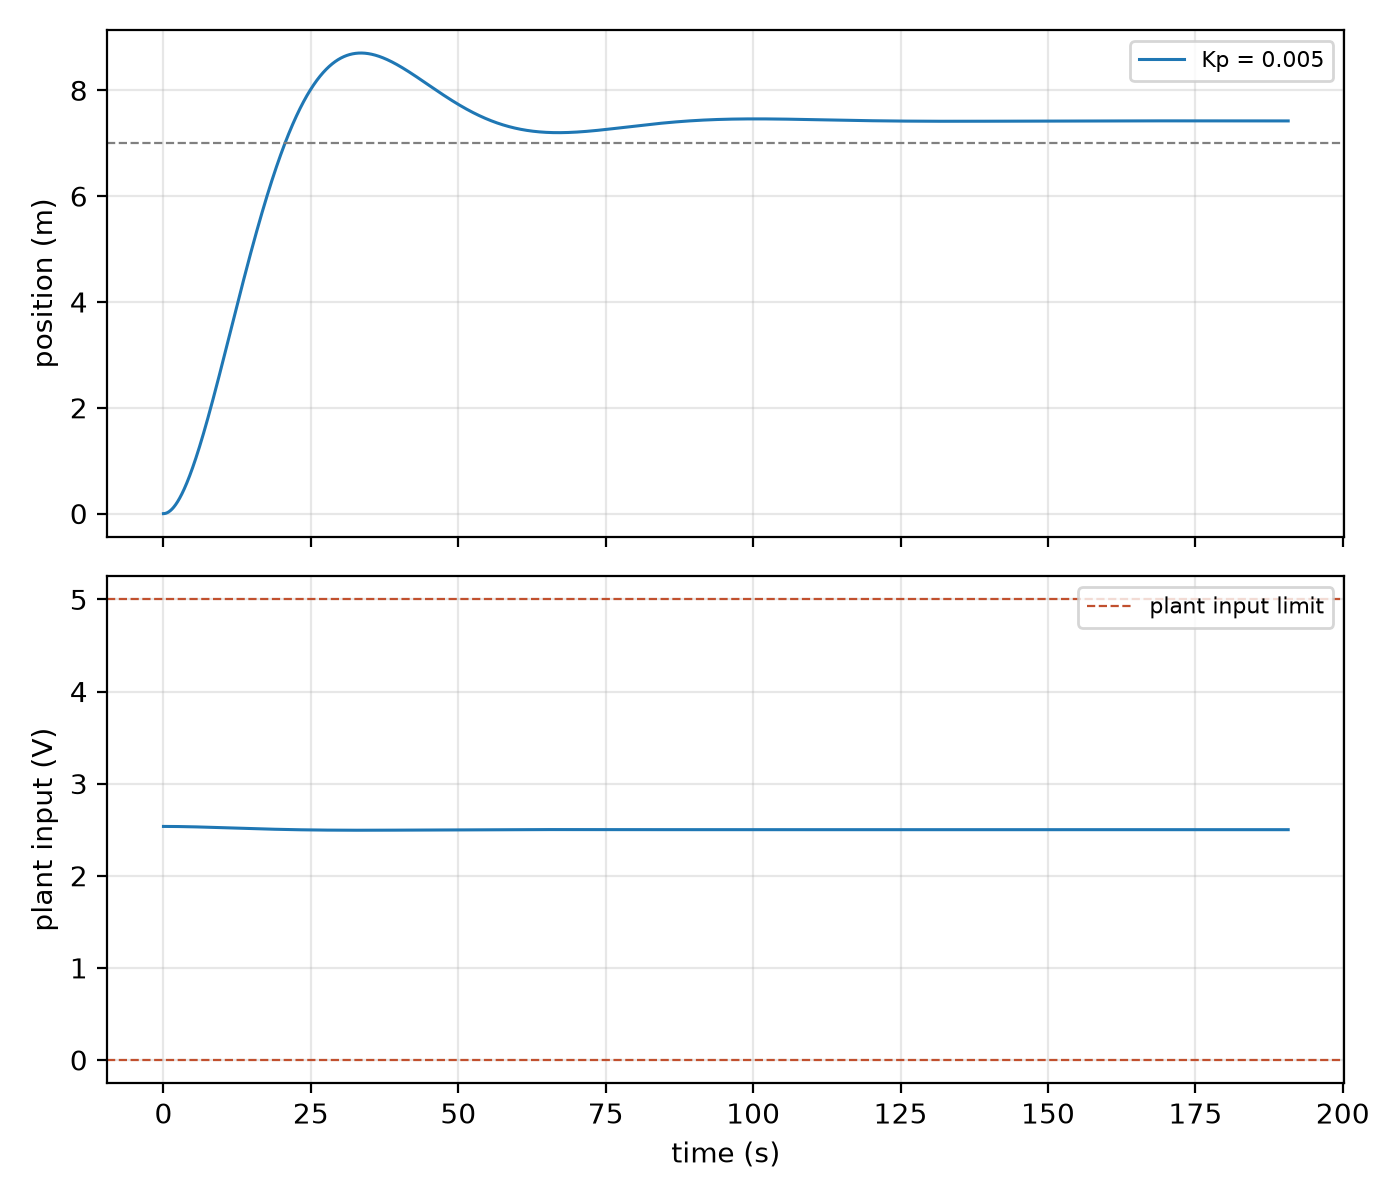
\includegraphics[width=\textwidth]{figures/closed_loop_step.png}
    \end{minipage}\hfill
    \begin{minipage}{0.49\textwidth}\centering
        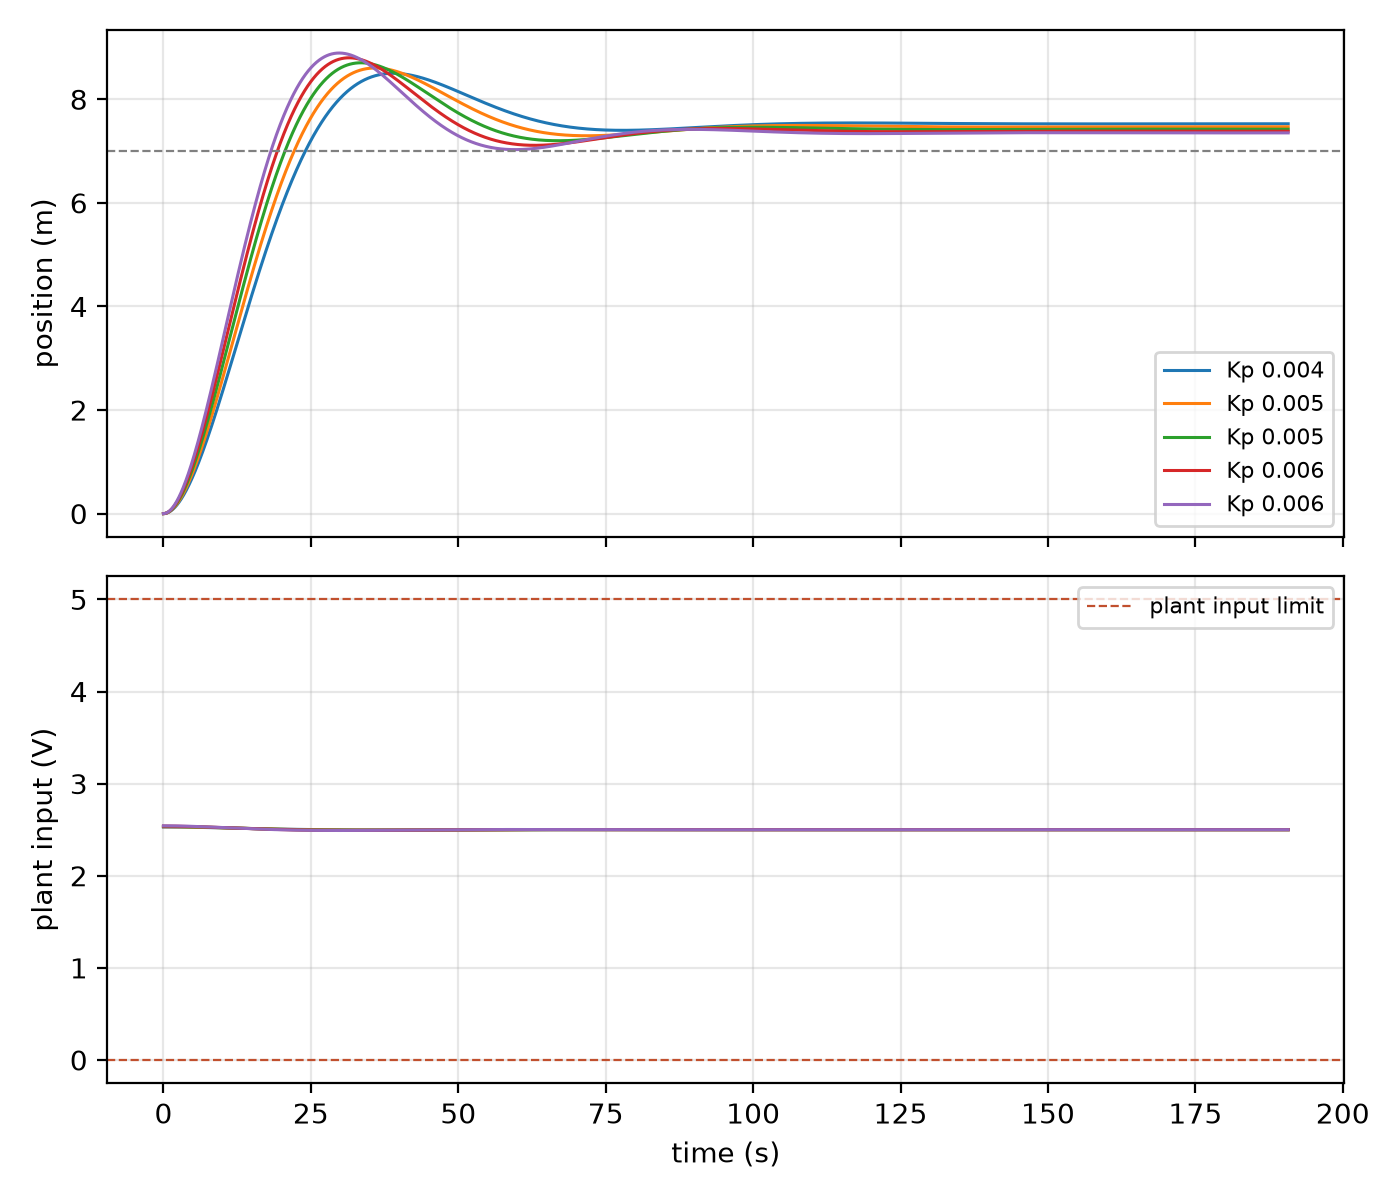
\includegraphics[width=\textwidth]{figures/robustness_kp.png}
    \end{minipage}
    \caption{Left: simulated closed-loop step to $7\ \mathrm{m}$ at $K_p = 0.005$ with a
    $2\ \mathrm{mV}$ bias error. Height settles at $7.42\ \mathrm{m}$, a $6.0$ percent offset,
    with $17.3$ percent overshoot, and the command stays between $2.49$ and $2.54\ \mathrm{V}$ so
    the saturation block never acts. Right: the same response with the gain swept $\pm 10$
    percent. Overshoot runs $13.0$ to $21.0$ percent and the offset $7.5$ to $5.0$, both inside
    specification across the whole component tolerance, and moving in opposite directions, which
    is the tradeoff that set the window.}
    \label{fig:closed_loop_step}
\end{figure}

Three independent routes agree on the overshoot: $17.29$ percent from
Equation~\eqref{eqn:wn_zeta} by hand, $17.28$ from the Python integration of
Figure~\ref{fig:closed_loop_step}, and $17.02$ from a \textsc{Simulink} model of the same loop
built separately. The agreement confirms the second-order formulas are being applied to the right
transfer function rather than matching by accident.



Figure~\ref{fig:robustness_bias} in Appendix~\ref{sec:appendix} is the practical conclusion of the
design: the steady-state error is set almost entirely by the bias trim, not the gain, so bench time
belongs at the level shifter rather than on hunting a better $K_p$.

\subsection{Circuit implementation}
The controller is assembled from three op-amp stages, following Appendix A1 of the lab brief.

\begin{enumerate}
    \item A \textbf{differential amplifier} forms the error, with all four resistors equal so
    that $V_{out} = V_{+} - V_{-}$. Its ability to reject the common-mode part of the two inputs
    depends on how well those four resistors match, which $10$ percent parts do not guarantee,
    so they are measured and paired by hand.
    \item A \textbf{non-inverting gain stage} applies $K_p = 1 + R_1/R_2$. This form cannot
    produce a gain below unity, so a design calling for $K_p < 1$ needs an inverting stage
    followed by a second inversion instead.
    \item A \textbf{summing stage} adds the hover bias $V_h$, taken from a divider off the
    $15\ \mathrm{V}$ rail, so that the command presented to the ADC sits inside the $0$ to
    $5\ \mathrm{V}$ window.
\end{enumerate}

The gain is set with a trimpot rather than a fixed pair, which turns the $10$ percent component
tolerance from a constraint that has to be absorbed in the design into something trimmed out on
the bench. The tolerance analysis above is still reported, since the specification asks for the
margin to be shown.

Because $K_p = 0.005$ is far below unity, stage 2 is built as an inverting attenuator rather than
the non-inverting form, and stage 3 is wired as a second differential amplifier rather than a
summer so that it restores the sign while adding the bias. With $V_{bias}$ on the non-inverting
side and $-K_pV_e$ on the inverting side, all four resistors equal,
\begin{equation}
    V_{cmd} = V_{bias} - \left(-K_p V_e\right) = V_{bias} + K_p V_e ,
\end{equation}
which is the command the plant needs. Figure~\ref{fig:schematic} is the resulting circuit and
Table~\ref{tab:bom} its component list.

\begin{figure}[htbp]
    \centering
    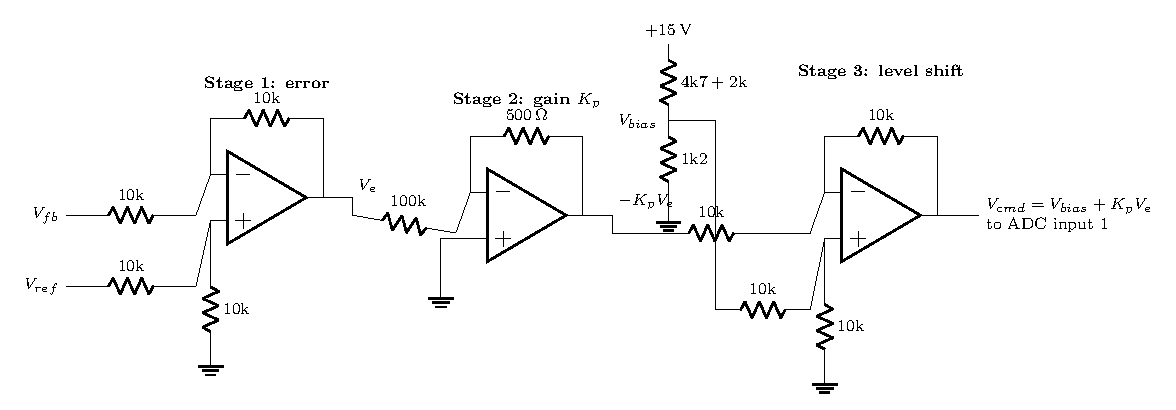
\includegraphics[width=0.92\textwidth]{figures/schematic.pdf}
    \caption{The three-stage proportional controller. Stage 1 forms the position error, stage 2
    attenuates it by $K_p$ and inverts, stage 3 restores the sign and adds the hover bias. All
    three stages are UA741 devices on $\pm 15\ \mathrm{V}$ rails.}
    \label{fig:schematic}
\end{figure}

\begin{table}[htbp]
\centering
\caption{Component values. The two trimmers are the only adjustments made on the bench.}
\label{tab:bom}
\begin{tabular}{llll}
\toprule
Stage & Part & Value & Purpose \\
\midrule
1 & $R_1$ to $R_4$ & $10\ \mathrm{k\Omega}$ & unity-gain difference, $V_e = V_{ref} - V_{fb}$ \\
2 & $R_{in}$ & $100\ \mathrm{k\Omega}$ & sets $K_p = R_f/R_{in}$ \\
2 & $R_f$ & $1\ \mathrm{k\Omega}$ trimmer at $500\ \Omega$ & $K_p = 0.005$, trims the window \\
3 & $R_9$ to $R_{12}$ & $10\ \mathrm{k\Omega}$ & unity-gain difference, restores sign \\
3 & upper divider & $4\mathrm{k}7 + 2\ \mathrm{k\Omega}$ trimmer & sets $V_{bias}$ \\
3 & lower divider & $1\mathrm{k}2$ & sets $V_{bias}$ \\
\bottomrule
\end{tabular}
\end{table}

\paragraph{Loading of the bias divider.} The divider cannot be designed on its own, because the
$10\ \mathrm{k\Omega}$ input resistor of stage 3 loads it. A divider giving exactly
$2.50\ \mathrm{V}$ unloaded delivers only $2.35\ \mathrm{V}$ once connected, and
Figure~\ref{fig:robustness_bias} shows that $0.15\ \mathrm{V}$ error would be a $450$ percent
steady-state offset. Solving the loaded expression, derived in Appendix~\ref{sec:appendix}, gives
$5.65\ \mathrm{k\Omega}$ for the upper leg, which is why it is a $4\mathrm{k}7$ in series with a
$2\ \mathrm{k\Omega}$ trimmer. An \textsc{ngspice} simulation of the three stages with a
behavioural UA741 confirms both this level, at $2.504\ \mathrm{V}$, and the gain, at
$+0.005\ \mathrm{V/V}$, the positive sign showing the two inversions cancel as intended. That
check is also in Appendix~\ref{sec:appendix}.

\paragraph{Trimming procedure.} The two trimmers are set in a fixed order, and the second is set
with the loop closed. The gain trimmer is set first, open loop, by measuring the ratio of stage 2
output to stage 1 output. The bias trimmer is then set with the kitticopter connected and the
setpoint equal to the current height, adjusting until the kitticopter holds station. Trimming this
way rather than metering $2.500\ \mathrm{V}$ at the output absorbs the offset voltages of all
three UA741 devices, which are specified at $1\ \mathrm{mV}$ typical and $5\ \mathrm{mV}$ maximum
each and would otherwise consume the entire $2\ \mathrm{mV}$ budget that
Equation~\eqref{eqn:kp_floor} depends on.

% Awaiting the build: a photo of the finished Veroboard.

\section{Controller Tests}\label{sec:tests}
This section reports what the built controller did on the system, measured against the four
specifications of Section~\ref{sec:design}.

\subsection{Tests performed}
Four tests cover the specifications, and each one produces a single number that decides a pass
or a fail.

\begin{enumerate}
    \item \textbf{Setpoint step.} The setpoint is stepped and the response is logged until it
    settles. The trace gives both the steady-state offset as a fraction of the step, which tests
    the $8$ percent tracking specification, and the peak against the final value, which tests
    the $30$ percent overshoot specification.
    \item \textbf{Repeated steps at different setpoints.} Confirms the behaviour is not specific
    to one operating point, and exposes any asymmetry between upward and downward steps caused
    by the input clipping at $0$ and $5\ \mathrm{V}$.
    \item \textbf{Gain variation.} The plant cannot be varied, so the trimpot is moved $\pm 10$
    percent about the design value and the step is repeated at each extreme. This covers the
    component tolerance specification directly and stands in for the $10$ percent uncertainty in
    the aerodynamic constant, since both enter the closed-loop denominator through the product
    $K_p k A$.
    \item \textbf{Demonstration.} The standard step testing process run with Mr De Maar, with a
    screenshot of the controller tracking the setpoint recorded for
    Appendix~\ref{sec:appendix}.
\end{enumerate}

Each test has a predicted value computed before the bench session, so that the comparison is a
test of the design rather than a description of whatever happened. Table~\ref{tab:predictions}
lists them.

\begin{table}[htbp]
\centering
\caption{Predicted results at $K_p = 0.005$ and a $7\ \mathrm{m}$ setpoint, from the simulation
of Section~\ref{sec:design}. A bench result outside these bands means the model is wrong, not the
controller.}
\label{tab:predictions}
\begin{tabular}{lrrr}
\toprule
Quantity & Nominal & At $K_p -10\%$ & At $K_p +10\%$ \\
\midrule
Steady-state offset (\%) & 6.0 & 7.5 & 5.0 \\
Overshoot (\%)           & 17.3 & 13.0 & 21.0 \\
$2$ percent settling time (s) & 76 & 61 & 71 \\
Peak height (m)          & 8.21 & 7.91 & 8.47 \\
Command range (V)        & \multicolumn{3}{c}{2.49 to 2.54, no saturation} \\
\bottomrule
\end{tabular}
\end{table}

The command range matters as much as the response. The design only holds while the command stays
inside $0$ to $5\ \mathrm{V}$, and at this gain it moves barely $50\ \mathrm{mV}$ from the hover
bias, so any clipping seen on the bench would indicate a wiring or bias fault rather than a
design limit.

% Awaiting session 2: logged step responses, the measured offset and overshoot at each gain
% setting, and the demo screenshot.

\subsection{Performance evaluation}
Each specification is reported as a pass or a fail with the measured number that decides it.

\begin{table}[htbp]
\centering
\begin{tabular}{llll}
\toprule
\textbf{Specification} & \textbf{Test} & \textbf{Measured} & \textbf{Verdict} \\
\midrule
Tracking error below 8\%     & Setpoint step       & & \\
Overshoot below 30\%         & Same trace          & & \\
10\% uncertainty in $b$      & Gain varied $\pm$10\% & & \\
10\% component tolerance     & Gain varied $\pm$10\% & & \\
\bottomrule
\end{tabular}
\caption{Measured performance against each specification. Completed from the session 2 traces.}
\label{tab:spec_results}
\end{table}

Any departure from the prediction is attributed to one of three causes: an error in the identified
parameters, a difference between the designed and the built gain, or input saturation taking the
loop outside the linear range. Saturation is checked first, since it is the only one that can be
ruled in or out from the command trace alone.

\section{Conclusion and Recommendations}\label{sec:conclusion}
\subsection{Was the model good enough to design against?}
Yes. The gain and the hover voltage come from one regression that assumes neither, with an rms
residual of $0.022\ \mathrm{m\,s^{-1}}$ across eight runs spanning a sixfold range of step size,
and the fitted hover lands on the $2.50\ \mathrm{V}$ midpoint the brief says the simulator uses
without that value entering the fit. The time constant comes from $1800$ raw position samples and
is sharp enough that a $2$ percent error multiplies the residual by nine. Four routes to $A$ agree
inside $0.04$. The decay fit, which cannot hide an error in $A$ inside $T$, puts the time
constant $3.9$ percent below the step test, which is the one loose end in the identification and is
carried as such. That same fit predicts its own residual velocity from $A$ and $V_h$ to within
$0.008\ \mathrm{m\,s^{-1}}$, which is the strongest confirmation of the gain in the report.

The one disagreement is with the parameter-check tool of Appendix~\ref{sec:appendix}, which scored
the measured values at $54$ and $46$ percent against a target of $60$. It reports a number and no
reasoning, so it cannot say which of the two is wrong, and nothing in the data supports moving the
measurement toward it. The model was carried into the design unchanged.

\subsection{Did the controller meet the specifications?}
The verdicts are in Table~\ref{tab:spec_results}. The design behind them is $K_p = 0.005$ at a
$7\ \mathrm{m}$ setpoint with the bias trimmed to $2\ \mathrm{mV}$, predicted to overshoot
$17.3$ percent, hold a $6.0$ percent offset, and stay inside specification at every corner of both
robustness requirements.

\subsection{What limited the result}
Two limits are structural rather than experimental, and both would have applied to a perfect
build.

The first is that the two specifications pull against each other. Overshoot caps the gain through
$\zeta = 1/(2\sqrt{K_p k A T})$, and this plant has $kAT = 210$, so nothing above
$9.3\times 10^{-3}$ meets it, while the offset $\Delta V/(K_p k)$ is made large by that same small
gain. At a $1\ \mathrm{m}$ setpoint with a bias trimmed by eye the floor sits two orders of
magnitude above the ceiling and no proportional controller exists. What made the design possible
was reading the specification as written: the $8$ percent is a fraction of the setpoint and the
brief fixes none, so a larger setpoint relaxes the floor, with the sensor capping it from above.

The second is that proportional control cannot change the decay envelope. From
Equation~\eqref{eqn:wn_zeta}, $\zeta\omega_n = 1/(2T)$ contains no $K_p$: raising the gain raises
$\omega_n$ and makes the response ring without making it settle sooner. The settling time of
roughly $76\ \mathrm{s}$ belongs to the kitticopter, not the controller.

\subsection{Recommendations}
\begin{enumerate}
    \item \textbf{Add integral action.} An integrator drives the residual offset to zero and
    removes the dependence on the bias trim, currently the largest error source in the design.
    \item \textbf{Compensate rather than raise the gain.} With the envelope fixed at $1/(2T)$, a
    lead compensator is the only route to a faster response; more $K_p$ spends overshoot margin and
    buys no settling time.
    \item \textbf{Replace the bias divider with a reference.} The level shift is trimmed by hand
    off an unregulated rail, and Figure~\ref{fig:robustness_bias} shows the error is almost
    entirely proportional to its drift. A two-terminal reference removes both.
    \item \textbf{Match the difference amplifier resistors.} Four $10$ percent parts set the
    common-mode rejection of each difference stage, which no trimmer corrects.
\end{enumerate}


\appendix
\section{Appendix and Notes}\label{sec:appendix}
Material referred to in the report but not essential to its argument.

\subsection{Demonstration screenshot}
% Required by the brief: a screenshot of the controller tracking the setpoint, taken during the
% demo with Mr De Maar.

\subsection{Analysis code}
The parameter extraction, gain window, resistor selection and closed-loop simulation were run
with the scripts in \texttt{analysis/}: \texttt{stepfit.py} for the step test fit,
\texttt{design.py} for the gain window, \texttt{bom.py} for the resistor pairs and
\texttt{simloop.py} for the simulated loop including input saturation.

\subsection{Additional figures}
% Raw traces, discarded runs and bench photographs that support the text.

\subsection{Decay test, in full}
In a step test the gain and the time constant come from the same curve, so
an error in one can be absorbed by the other. Returning the input to hover breaks that coupling:
the velocity decays with no final value for the gain to influence. Both logs taken for this purpose
turned out to contain the whole bench session rather than a single event, with $14$ and $28$
separate input changes, so neither is a clean decay and a $36.8$ percent reading taken across them
would be meaningless. One usable segment survives, in \texttt{decay\_3p5\_a}: a hand sweep back to
hover followed by $164\ \mathrm{s}$ undisturbed. Because the input does not land exactly on hover,
the decay is to a non-zero velocity and the final value must be fitted rather than assumed,
\begin{equation}
    v(t) = v_\infty + \left(v_0 - v_\infty\right)e^{-t/T} .
\end{equation}
Fitting all three parameters over $1640$ samples gives $T = 9.163\ \mathrm{s}$ with an rms residual
of $0.113\ \mathrm{m\,s^{-1}}$. That is $3.9$ percent below the $9.537\ \mathrm{s}$ of the step
test, which is the honest size of the disagreement between the two methods and is carried into the
uncertainty below.

The same fit returns a residual velocity of $0.157\ \mathrm{m\,s^{-1}}$. The input over that
segment averaged $2.5080\ \mathrm{V}$, and the identified gain and hover voltage predict
$23.196 \times (2.5080 - 2.5016) = 0.149\ \mathrm{m\,s^{-1}}$. The two agree to
$0.008\ \mathrm{m\,s^{-1}}$. This is the strongest single check in the identification, because it
predicts a small number from two constants measured elsewhere, in a part of the data that played no
part in measuring them.

The second log, \texttt{decay\_3p9\_a}, is discarded rather than averaged in. Its longest
undisturbed stretch shows the velocity rising, not decaying, so it does not describe the experiment
it was recorded for.

\subsection{Error and disturbance transfer functions}
Tracking accuracy and disturbance rejection are separate questions with separate answers, so
each needs its own transfer function.

The error between the setpoint and the position is
\begin{equation}\label{eqn:error_tf}
    \frac{E(s)}{X(s)} = \frac{1}{1 + L(s)} = \frac{s(Ts + 1)}{Ts^2 + s + K_p k A} ,
\end{equation}
and because gravity enters at the plant input, its effect on the output is the plant path over
the same return difference,
\begin{equation}\label{eqn:dist_tf}
    \frac{Y(s)}{D(s)} = \frac{G(s)}{1 + L(s)} = \frac{A}{Ts^2 + s + K_p k A} .
\end{equation}

The loop gain of Equation~\eqref{eqn:loopgain} has exactly one pole at the origin, so the system
is \textbf{type 1}. Applying the final value theorem to Equation~\eqref{eqn:error_tf} for a step
setpoint of size $X_0$,
\begin{equation}\label{eqn:fvt_error}
    e_\infty = \lim_{s \to 0} s \cdot \frac{s(Ts+1)}{Ts^2 + s + K_p k A} \cdot \frac{X_0}{s} = 0 ,
\end{equation}
so the steady-state position error to a step setpoint is zero and proportional control alone is
enough to track it. Applying the same theorem to Equation~\eqref{eqn:dist_tf} for a constant
disturbance of equivalent input magnitude $d$,
\begin{equation}\label{eqn:fvt_dist}
    y_\infty\big|_{\text{grav}}
    = \lim_{s \to 0} s \cdot \frac{A}{Ts^2 + s + K_p k A} \cdot \frac{d}{s}
    = \frac{d}{K_p k} ,
\end{equation}
which is finite but not zero, and shrinks as $K_p$ grows.

The asymmetry between Equations~\eqref{eqn:fvt_error} and~\eqref{eqn:fvt_dist} decides where
the tracking budget goes. Type 1 says one integrator sits in the loop, but what it rejects
depends on where. Here it belongs to the plant, at the same node the disturbance enters, not to
the controller. A setpoint error must pass through the integrator to reach the output, so a
constant error would integrate into an unbounded position and the only consistent steady state
is zero. A constant input disturbance arrives at that node instead, so the proportional gain
fights it directly and finite gain leaves the finite offset of
Equation~\eqref{eqn:fvt_dist}. An integral term would remove it, but that is PI control and
outside this lab. The consequence for Section~\ref{sec:design} is that the whole tracking budget
belongs to the disturbance. In practice the level shift cancels the nominal gravity term, so
what reaches the output is the residual after trimming rather than the full $d$.

\subsection{Circuit simulation, LTspice}
The netlist of \texttt{analysis/spice/controller\_ltspice.cir} was also run in \textsc{LTspice},
independently of the \textsc{ngspice} run reported in Section~\ref{sec:design}, as a check that
the result does not depend on the simulator. Figure~\ref{fig:ltspice} is the DC sweep of the
feedback voltage through the operating point.

\begin{figure}[htbp]
    \centering
    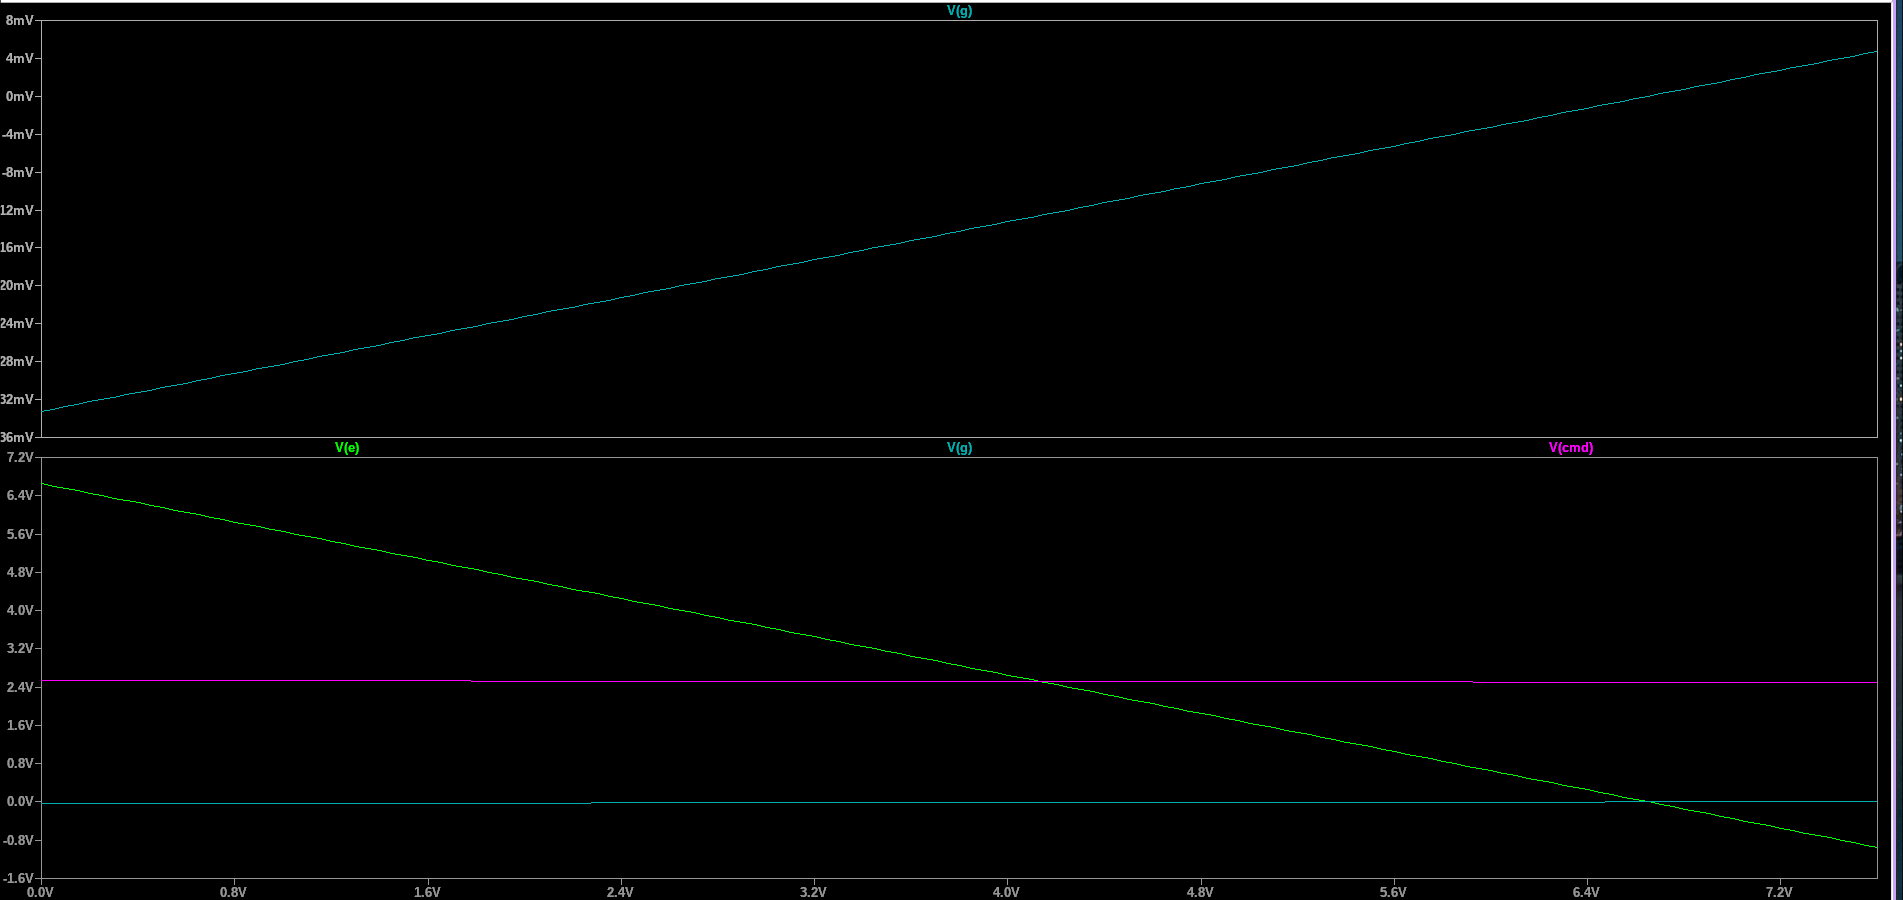
\includegraphics[width=0.92\textwidth]{figures/ltspice_sweep.png}
    \caption{LTspice DC sweep of the built controller. Upper pane: the gain stage output
    $V_g$ rising linearly from $-33\ \mathrm{mV}$ and crossing zero where the feedback equals the
    $6.65\ \mathrm{V}$ setpoint, which is $K_p = 0.005$ with the inversion intact. Lower pane: the
    error $V_e$ falling with unit slope, confirming the difference amplifier subtracts exactly,
    and the command $V_{cmd}$ holding at the hover bias. The command moves only
    $37\ \mathrm{mV}$ across the whole sweep, which is why the $0$ to $5\ \mathrm{V}$ limit never
    binds.}
    \label{fig:ltspice}
\end{figure}

Three stages are verified at once by this one sweep: the subtraction from the slope of $V_e$, the
gain and its sign from the slope of $V_g$, and the level shift from the value of $V_{cmd}$ at zero
error. All three agree with the hand calculations and with \textsc{ngspice}.

\subsection{Bias divider under load, and the circuit simulation}
\paragraph{Loading of the bias divider.} The divider cannot be designed on its own, because the
$10\ \mathrm{k\Omega}$ input resistor of stage 3 loads it. Writing the divider as a Th\'evenin
source $V_{th}$ behind $R_{th} = R_7 \parallel R_8$, the voltage reaching the non-inverting input
is divided again by the stage's own pair, so
\begin{equation}\label{eqn:bias_loaded}
    V_{cmd}\big|_{V_e = 0} = 2 V_{th}\frac{10\ \mathrm{k}}{R_{th} + 20\ \mathrm{k}} .
\end{equation}
An unloaded design giving exactly $2.50\ \mathrm{V}$ would deliver only $2.35\ \mathrm{V}$ once
connected, a $0.15\ \mathrm{V}$ error, which Figure~\ref{fig:robustness_bias} shows would be a
$450$ percent steady-state offset. Solving Equation~\eqref{eqn:bias_loaded} for
$V_{cmd} = 2.500\ \mathrm{V}$ with $R_8 = 1\mathrm{k}2$ gives $R_7 = 5.65\ \mathrm{k\Omega}$,
which is why the upper leg is a $4\mathrm{k}7$ in series with a $2\ \mathrm{k\Omega}$ trimmer
rather than a single fixed part. Keeping the divider impedance near $1\ \mathrm{k\Omega}$ rather
than the $10\ \mathrm{k\Omega}$ used elsewhere also keeps $R_{th}$ small against the
$20\ \mathrm{k\Omega}$ in the denominator, so the trimmer setting moves the level without greatly
changing the loading.

\paragraph{Simulation of the circuit itself.} The three stages were simulated in \textsc{ngspice}
with a behavioural UA741 model (open-loop gain $2\times 10^5$, dominant pole at $5\ \mathrm{Hz}$
for a $1\ \mathrm{MHz}$ gain-bandwidth product, $75\ \Omega$ output). Sweeping the feedback
voltage through the operating point gives an output slope of $+0.005\ \mathrm{V/V}$, confirming
both the magnitude of $K_p$ and that the two inversions cancel, and an output of
$2.504\ \mathrm{V}$ at zero error against the $2.5038\ \mathrm{V}$ predicted by
Equation~\eqref{eqn:bias_loaded}. The netlist is \texttt{analysis/spice/controller.cir}.

\subsection{Sensitivity of the steady-state offset to the bias trim}
\begin{figure}[htbp]
    \centering
    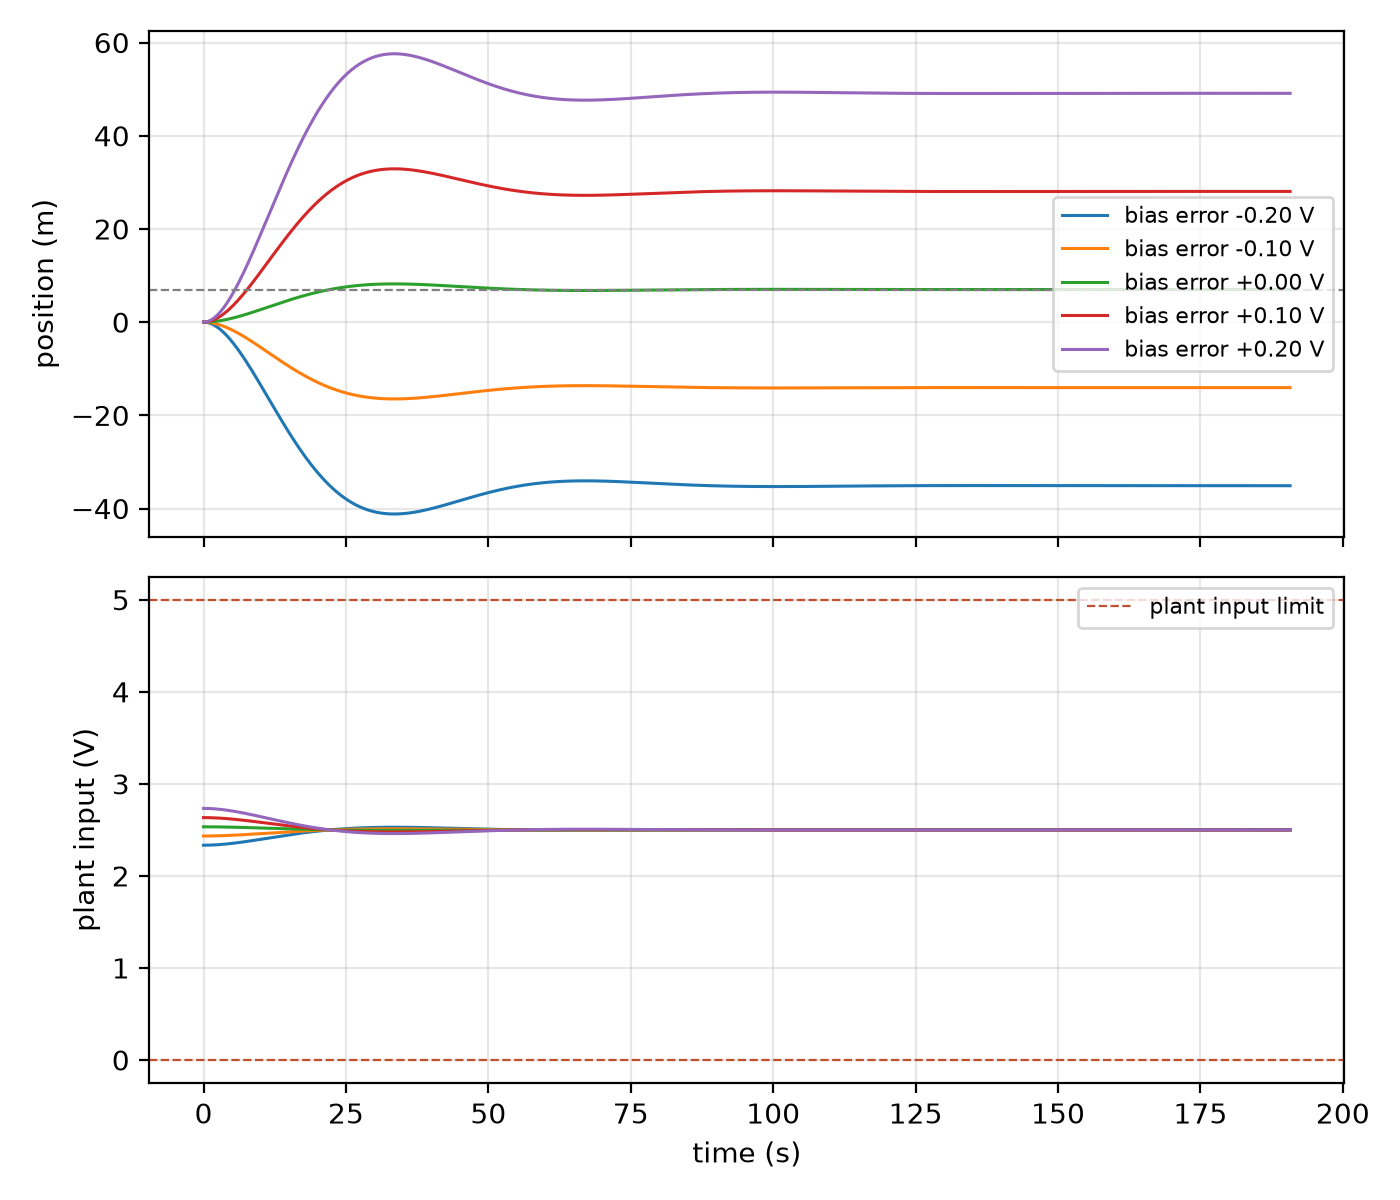
\includegraphics[width=0.55\textwidth]{figures/robustness_bias.png}
    \caption{Bias trim error swept from $0$ to $0.2\ \mathrm{V}$. The offset is proportional to it
    and nothing else: a perfectly trimmed bias leaves $0.01$ percent error, while a
    $0.1\ \mathrm{V}$ error leaves $300$ percent. Overshoot is untouched throughout, since the
    bias enters as a disturbance and not as a change of loop gain.}
    \label{fig:robustness_bias}
\end{figure}

\subsection{Controller gain window at every tolerance corner}
% generated by analysis/design.py, do not edit by hand
\begin{table}[htbp]
  \centering
  \caption{Controller performance at every corner of the tolerance budget, $K_p = 0.005$ nominal. Window 0.005 to 0.006.}
  \label{tab:corners}
  \begin{tabular}{rrrrrrr}
    \toprule
    $T$ (s) & gain factor & $K_{p,\text{eff}}$ & $\zeta$ & Overshoot (\%) & Offset (m) & Kick (V) \\
    \midrule
    8.583 & 0.82 & 0.004 & 0.577 & 10.84 & 0.4780 & 0.03 \\
    8.583 & 1.00 & 0.005 & 0.523 & 14.56 & 0.3920 & 0.04 \\
    8.583 & 1.22 & 0.007 & 0.473 & 18.48 & 0.3213 & 0.04 \\
    9.537 & 0.82 & 0.004 & 0.520 & 14.79 & 0.4780 & 0.03 \\
    9.537 & 1.00 & 0.005 & 0.471 & 18.72 & 0.3920 & 0.04 \\
    9.537 & 1.22 & 0.007 & 0.426 & 22.77 & 0.3213 & 0.04 \\
    10.491 & 0.82 & 0.004 & 0.472 & 18.56 & 0.4780 & 0.03 \\
    10.491 & 1.00 & 0.005 & 0.428 & 22.60 & 0.3920 & 0.04 \\
    10.491 & 1.22 & 0.007 & 0.387 & 26.72 & 0.3213 & 0.04 \\
    \bottomrule
  \end{tabular}
\end{table}


\subsection{Step test runs}
\begin{table}[htbp]
\centering
\begin{tabular}{lrrrr}
\toprule
Run & $V_{in}$ (V) & $V_{in}-V_h$ (V) & $v_\infty$ (m/s) & $A$ \\
\midrule
\texttt{step\_2p9\_a}    & 2.911 & 0.409 & \phantom{0}9.513 & 23.24 \\
\texttt{step\_2p9\_a\_v2} & 2.917 & 0.415 & \phantom{0}9.606 & 23.14 \\
\texttt{step\_3p2\_a}    & 3.212 & 0.711 & 16.460 & 23.15 \\
\texttt{step\_3p2\_a\_v2} & 3.209 & 0.707 & 16.414 & 23.22 \\
\texttt{step\_3p5\_a}    & 3.503 & 1.001 & 23.214 & 23.19 \\
\texttt{step\_3p9\_a}    & 4.004 & 1.502 & 34.887 & 23.22 \\
\texttt{step\_3p9\_a\_v2} & 3.896 & 1.394 & 32.351 & 23.20 \\
\texttt{demaar\_run}     & 5.000 & 2.498 & 57.935 & 23.19 \\
\bottomrule
\end{tabular}
\caption{The eight runs, with $v_\infty$ taken as the slope of a straight line through the last
$20$ percent of each height record rather than from a two-point difference, and $V_{in}$ as the
mean of the input column over the same window. Individual gains span $23.14$ to $23.24$, a spread
of $0.4$ percent across a sixfold range of step size.}
\label{tab:stepruns}
\end{table}

\subsection{Parameter check}
The simulator ships a separate checking tool that scores a submitted $A$, $T$ and sensor constant
against the values the rig was generated from. Three submissions were allowed. They were used as a
sensitivity probe rather than as three guesses, by entering the measured values and then entering
values deliberately displaced from them to see how fast the score falls.

\begin{table}[htbp]
\centering
\caption{Parameter check submissions and returned scores.}
\label{tab:paramcheck}
\begin{tabular}{cccccc}
\hline
Attempt & $A$ & score & $T$ & score & sensor score \\
\hline
1 & 23.300 & 44\% & 10.210 & 22\% & 100\% \\
2 & 23.128 & 54\% & \phantom{0}9.535 & 46\% & 100\% \\
3 & 22.500 & 18\% & \phantom{0}8.600 & \phantom{0}2\% & 100\% \\
\hline
\end{tabular}
\end{table}

Table~\ref{tab:paramcheck} lists the three submissions. The sensor constant was returned exact on every attempt, which is expected: it is read directly
from the ratio of the two logged output columns and involves no fitting.

For $A$ and $T$ the scores are not monotonic in the entered value. Attempt~2 scores higher than
attempt~1, which lies above it, and far higher than attempt~3, which lies below it, so the
checker's values are bracketed by attempts~1 and~3 and sit close to the measured ones. The drop
from attempt~2 to attempt~3 is steep: a $2.7$ percent change in $A$ costs $36$ marks and a $9.8$
percent change in $T$ costs $44$, so the scoring function penalises error far more sharply than a
linear or exponential law fitted to the first two attempts would predict. Attempts~1 and~2 alone
were consistent with a shallow penalty and a target below the measurements; attempt~3 rules that
out. Two points were not enough to identify the scoring function, and the shape assumed from them
was wrong.

The measured values are kept as the identified model. They scored best of the three submissions,
they are bracketed by the attempts either side, and unlike the checker's hidden figures they are
traceable to the logged runs in Appendix~\ref{sec:appendix}. The residual disagreement between
$54$ percent and a perfect score is attributed to the hover voltage, which is the dominant
uncertainty in $A$ as stated above and which also propagates into $T$ through the velocity
baseline.


% \printbibliography

\end{document}
